% ----------------------------------------------------------
% 1 Introdução
% ----------------------------------------------------------

Em 2015, na sede da ONU de Nova Iorque, aconteceu um encontro entre todos os países das Nações 
Unidas, com o objetivo de traçar metas visando o desenvolvimento sustentável. Com isso, uma agenda 
foi desenvolvida e nomeada de Objetivos de Desenvolvimento Sustentável. 

Dentre os 17 objetivos identificados, o 11º é descrito como \"Tornar as cidades e os assentamentos 
humanos inclusivos, seguros, resilientes e sustentáveis", chamando a atenção para as taxas 
alarmantes de emissão de gases residuais principalmente em áreas urbanas. Em 2015 foi registrado que 
metade da população mundial vive em grandes cidades e a previsão para 2030 é que essa porcentagem 
suba para 60\%, ou seja, as cidades que ocupam aproximadamente apenas 2\% da área do planeta irão 
abrigar 60\% da humanidade, consumindo 80\% da energia produzida e causando 75\% da emissão de gases 
poluentes na atmosfera. 

No Brasil, o crescimento desgovernado nas metrópoles tem ameaçado a infraestrutura não planejada, 
enfatizando problemas como oferta de água potável, esgoto, saúde pública, transporte, qualidade do 
ar, conservação de energia, diminuição do impacto gerado pelo trânsito, dentre outros. Em 2016, 
segundo uma pesquisa implementada pela Organização Mundial da Saúde (OMS), 92\% da população mundial 
esteve exposta a níveis alarmantes de poluição e 7  milhões de pessoas morreram devido à degradação 
ambiental - sendo 4 milhões relacionadas ao uso da madeira, carvão e biomassa, e 3 milhões aos gases 
residuais liberados por veículos automotores. Surpreendentemente, esse número excede a quantidade de 
mortes por síndrome da imunodeficiência adquirida (do termo em inglês: \"Acquired Immunodeficiency 
Syndrome\" - AIDS) e malária juntos.

De acordo com a OMS, os problemas relacionados à exposição constante de poluentes são o AVC 
(Acidente Vascular Cerebral), problemas respiratórios, diabetes, doenças cardiovasculares, câncer e 
infertilidade. Tais problemas podem ser influenciados ou catalisados por compostos orgânicos 
voláteis, como tinta de parede, revestimento de carpete e produtos de limpeza, até os gases 
liberados pelas indústrias e veículos automotores.

Quando gases ou partículas emitidos pela ação humana atingem concentrações suficientemente altas que 
causam danos diretos à população, seja ela humana ou não, um requisito básico para o bem estar de 
todos é negligenciado.

O projeto estadual MonitorAR Rio coleta dados de emissão de gases poluentes desde 2010, nas regiões 
Centro, Copacabana, São Cristóvão, Tijuca, Irajá, Bangu, Campo Grande, Pedra de Guaratiba e Recreio. 
Em 2011 e 2012, os seguintes dados referentes a taxa de gases poluentes coletados foram:

\begin{figure*}
	\centering
	\begin{subfigure}{0.5\textwidth}
		\centering
		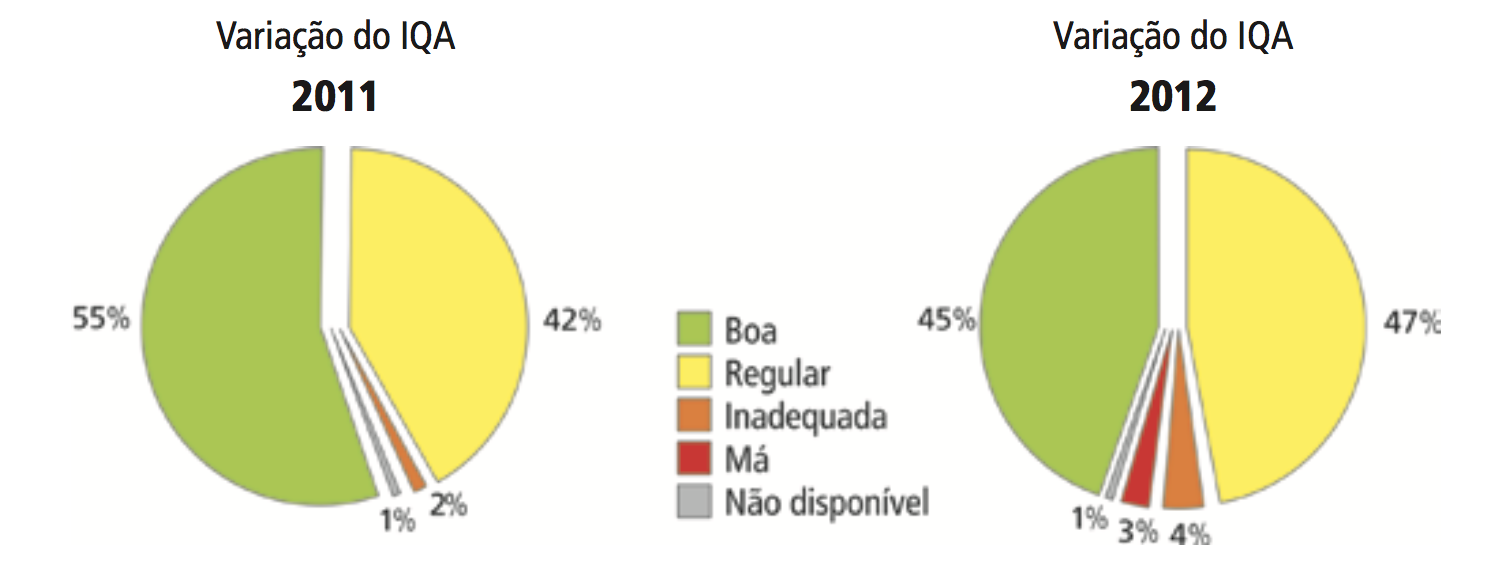
\includegraphics[scale=0.6]{chapter1-img1}
	\end{subfigure}
    \par
    \phantomcaption \small { 
        Gráfico com a variação do IQA 2011: 
        \par
        Bom 55\% | Regular 42\% | Inadequado 2\% | Ruim 0\% | Não disponível 1\% 
        \par
        Fonte: Relatório da Rede MonitorAr-Rio, 2011-2012 }
\end{figure*}

\begin{figure*}
	\centering
	\begin{subfigure}{0.5\textwidth}
		\centering
		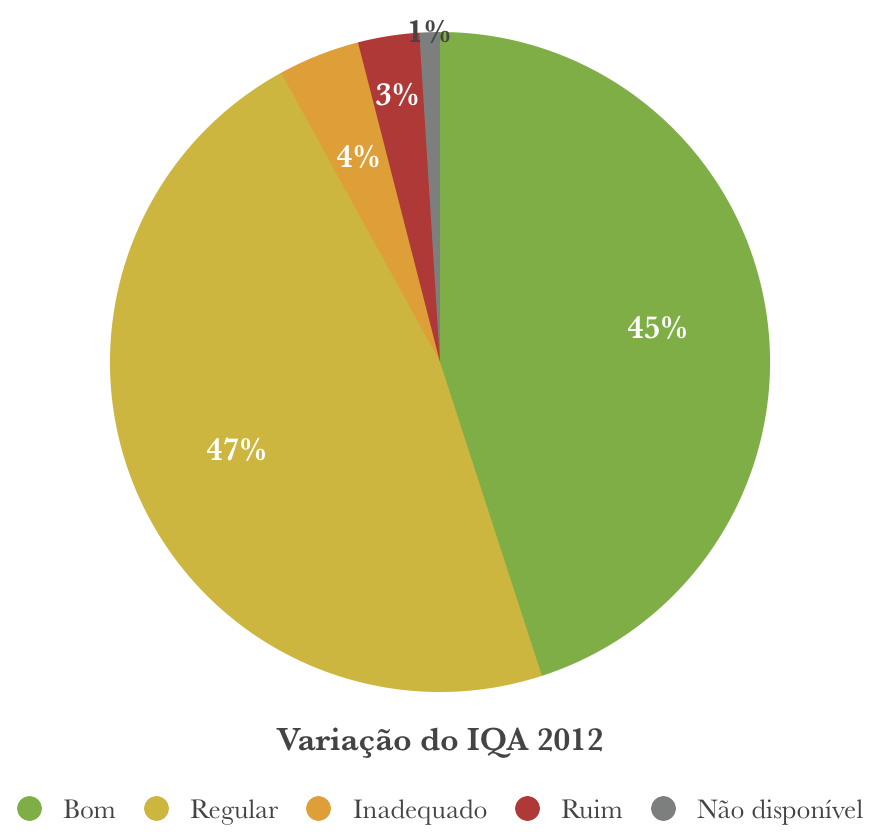
\includegraphics[scale=0.6]{chapter1-img2}
	\end{subfigure}
    \par
    \phantomcaption \small { 
        Gráfico com a variação do IQA 2012: 
        \par
        Bom 45\% | Regular 47\% | Inadequado 4\% | Ruim 3\% | Não disponível 1\%
        \par
        Fonte: Relatório da Rede MonitorAr-Rio, 2011-2012 }
\end{figure*}

\begin{figure*}
	\centering
	\begin{subfigure}{0.5\textwidth}
		\centering
		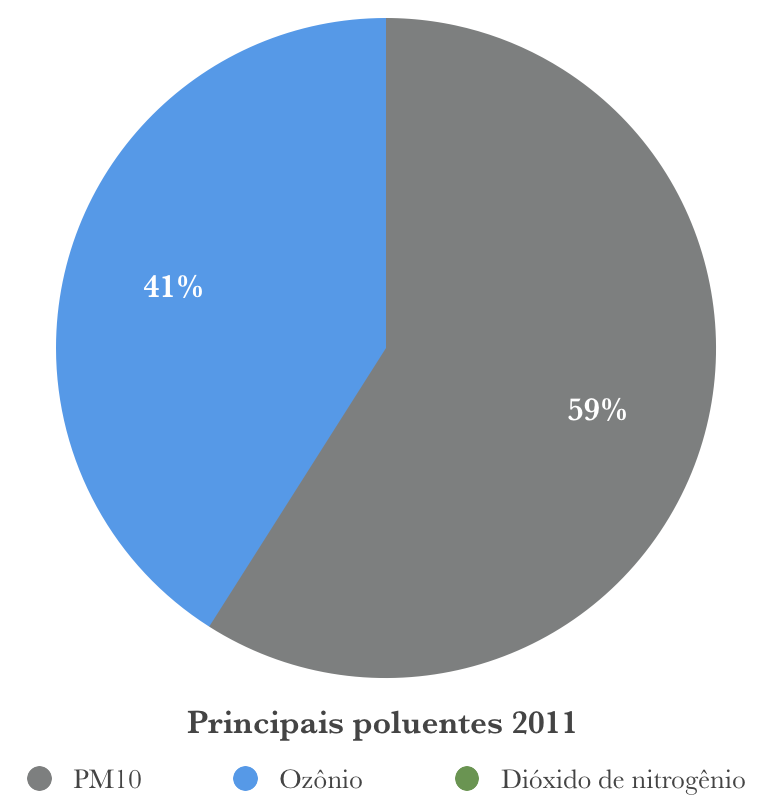
\includegraphics[scale=0.6]{chapter1-img3}
	\end{subfigure}
    \par
    \phantomcaption \small { 
        Gráfico com principais poluentes de 2011: 
        \par
        PM10 59\% | Ozônio 41\% | Dióxido de nitrogênio 0\%
        \par
        Fonte: Relatório da Rede MonitorAr-Rio, 2011-2012 }
\end{figure*}

\begin{figure*}
	\centering
	\begin{subfigure}{0.5\textwidth}
		\centering
		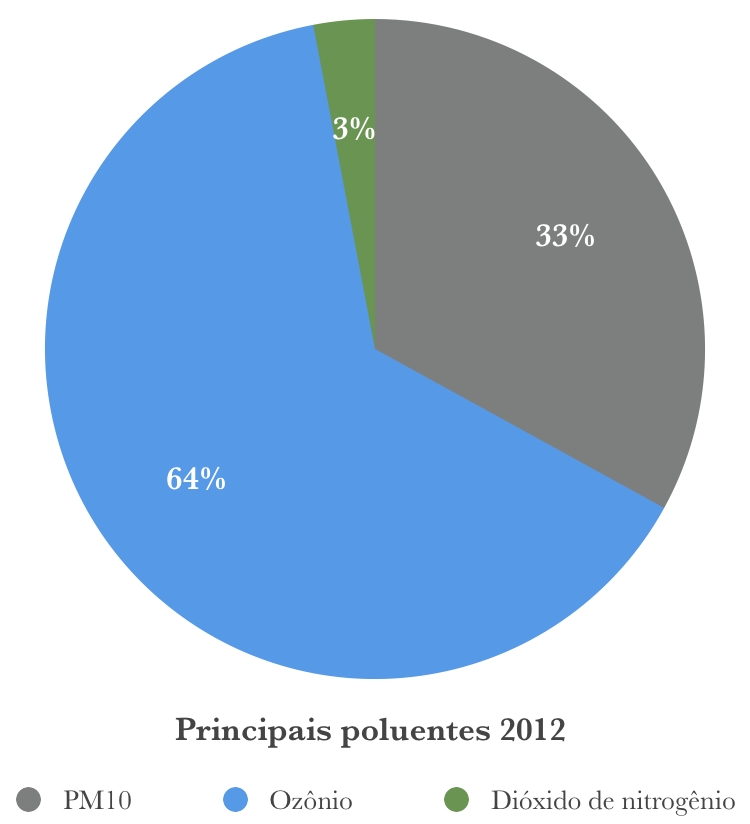
\includegraphics[scale=0.6]{chapter1-img4}
	\end{subfigure}
    \par
    \phantomcaption \small { 
        Gráfico com principais poluentes de 2012:
        \par
        PM10 33\% | Ozônio 64\% | Dióxido de nitrogênio 3\% 
        \par
        Fonte: Relatório da Rede MonitorAr-Rio, 2011-2012 }
\end{figure*}

Dentro dessa perspectiva, voltados para a questão da qualidade do ar e do impacto gerado pelo 
trânsito, urbanistas de todo o mundo se reuniram para discutir e desenvolver programas urbanísticos 
de baixo nível de agressão ambiental, bem como buscar definir um desenvolvimento socioeconômico que 
melhore e não destrua o meio ambiente natural e construído.

Algumas cidades europeias, percebendo a importância de transportes alternativos, priorizaram a 
bicicleta no trânsito, com a intenção de diminuir a poluição ambiental, humanizar as ruas e reduzir 
a quantidade de acidentes. Para isso o governo disponibilizou bicicletas públicas e investiu na 
construção de redes cicloviárias interligadas a outros transportes públicos, como metrô, barcas, 
trens e etc. No Brasil, um exemplo de programa semelhante é o BikeRio. Esse programa foi desenvolvido 
pelo governo do Rio de Janeiro em parceria com o Itaú, promovendo o aluguel de bicicletas por um 
valor mensal ou diário acessível. Ainda que o BikeRio seja um sucesso, o uso da bicicleta ainda 
encontra fortes obstáculos, especialmente por causa da falta de cidadania e respeito no trânsito e 
pelas ciclovias escassas e de má qualidade - mesmo em cidades como Curitiba e Rio de Janeiro, onde 
existe um investimento mais forte nesse contexto.

Além de usada como meio de transporte, a bicicleta é boa para a saúde, sendo considerada uma das 
melhores técnicas para prevenir e tratar a hipertensão, o infarto do miocárdio e o colesterol alto.

Este trabalho tem como objetivo mensurar a quantidade de ar poluído inalado, em média, pelo ciclista 
carioca das regiões urbanas. Um dispositivo embarcado será instalado na bicicleta, com a capacidade 
de captar o nível de gases poluentes durante o trajeto do ciclista. Os dados poderão ser consultados 
em tempo real através de uma página web.

Para alcançar este propósito, será criado um protótipo com o Arduino Trinket, principalmente por ser 
uma placa pequena, de fácil implementação e com diversas portas I/O, flexibilizando a inclusão dos 
sensores. O protótipo será planejado baseado em redes LoRa. Estas são redes sem fio de alto alcance 
e baixo consumo de energia, criadas especificamente para promover a comunicação entre dispositivos 
embarcados (IoT). Com isso, é possível acessar os dados captados por cada usuário em tempo real.

No capítulo 2, \"Resumo histórico e estado da arte", serão apresentadas diversas pesquisas referentes 
ao tema do trabalho, evidenciando as tecnologias e soluções encontradas até o presente momento, para 
mitigar os problemas relacionados; no capítulo 3 - \"Proposição do problema" - o problema, encontrado 
através das pesquisas, será brevemente descrito; e no capítulo 4 - \"Solução proposta" - a solução 
proposta será apresentada, abordando os aspectos tecnológicos e suas premissas, contendo uma visão 
geral do sistema a ser desenvolvido.

% TODO: Quando um novo capítulo for adicionado, adicionar a descrição aqui.